\documentclass[]{rptuseminar}

% Specify that the source file has UTF8 encoding
\usepackage[utf8]{inputenc}
% Set up the document font; font encoding (here T1) has to fit the used font.
\usepackage[T1]{fontenc}
\usepackage{lmodern}

% Load language spec
\usepackage[american]{babel}
% German article --> ngerman (n for »neue deutsche Rechtschreibung«)
% British English --> english

% Ffor bibliography and \cite
\usepackage{cite}

% AMS extensions for math typesetting
\usepackage[intlimits]{mathtools}
\usepackage{amssymb}
% ... there are many more ...


% Load \todo command for notes
\usepackage{todonotes}
% Sebastian's favorite command for large inline todonotes
% Caveat: does not work well with \listoftodos
\newcommand\todoin[2][]{\todo[inline, caption={2do}, #1]{
		\begin{minipage}{\linewidth-1em}\noindent\relax#2\end{minipage}}}

% Load \includegraphics command for including pictures (pdf or png highly recommended)
\usepackage{graphicx}

% Typeset source/pseudo code
\usepackage{listings}

% Load TikZ library for creating graphics
% Using the PGF/TikZ manual and/or tex.stackexchange.com is highly adviced.
\usepackage{tikz}
% Load tikz libraries needed below (see the manual for a full list)
\usetikzlibrary{automata,positioning}

% Load \url command for easier hyperlinks without special link text
\usepackage{url}

% Load support for links in pdfs
\usepackage{hyperref}

% Defines default styling for code listings
\definecolor{gray_ulisses}{gray}{0.55}
\definecolor{green_ulises}{rgb}{0.2,0.75,0}
\lstset{%
  columns=flexible,
  keepspaces=true,
  tabsize=3,
  basicstyle={\fontfamily{tx}\ttfamily\small},
  stringstyle=\color{green_ulises},
  commentstyle=\color{gray_ulisses},
  identifierstyle=\slshape{},
  keywordstyle=\bfseries,
  numberstyle=\small\color{gray_ulisses},
  numberblanklines=false,
  inputencoding={utf8},
  belowskip=-1mm,
  escapeinside={//*}{\^^M} % Allow to set labels and the like in comments
}

% Defines a custom environment for indented shell commands
\newenvironment{displayshellcommand}{%
	\begin{quote}%
	\ttfamily%
}{%
	\end{quote}%
}

%%%%%%%%%%%%%%%%%%%%%%%%%%%%%%%%%%%%%%%%%%%%%%%%%%%%%%%%%%%%%%%%%%%%%%%%%%%%%%%

\title{Liquid Haskell}
\event{Seminar: Programming Languages in Winter term 2024/2025}
\author{Mehran Shahidi, Saba Safarnezhad
  \institute{Rheinland-Pfälzische Technische Universität Kaiserslautern-Landau, Department of Computer Science}}

%%%%%%%%%%%%%%%%%%%%%%%%%%%%%%%%%%%%%%%%%%%%%%%%%%%%%%%%%%%%%%%%%%%%%%%%%%%%%%%
\begin{document}
%%%%%%%%%%%%%%%%%%%%%%%%%%%%%%%%%%%%%%%%%%%%%%%%%%%%%%%%%%%%%%%%%%%%%%%%%%%%%%%

\maketitle

%%%%%%%%%%%%%%%%%%%%%%%%%%%%%%%%%%%%%%%%%%%%%%%%%%%%%%%%%%%%%%%%%%%%%%%%%%%%%%%

\begin{abstract}
  This report gives a brief overview of Liquid Haskell, a tool that extends Haskell with refinement types. Refinement types are types that extends expressiveness of Haskell types systems by providing predicates that can verify
  invarients of the program. This report explains briefly how SMT solvers leveraged by Liquid Haskell and how to use Liquid Haskell by providing some examples. Finally, we also discuss the limitations of Liquid Haskell and compare it with other tools.
\end{abstract}

%%%%%%%%%%%%%%%%%%%%%%%%%%%%%%%%%%%%%%%%%%%%%%%%%%%%%%%%%%%%%%%%%%%%%%%%%%%%%%

\section{Introduction}
\label{sec:introduction}

% E.~g.~ 
% ``quoting'' is done by using two backticks and two single quotes

\section{Background}
\label{sec:relatedwork}

\section{Working with LiquidHaskell}
  \label{sec:solution}
  
  Whatever the addressed problem is: now the author can start to explain her/his work.
  After the explanation, experiences, results or just a discussion of the presented work has to be given in Section \ref{sec:conclusions}.
  
\section{Example Application}

\todo{ state the problem}
\todo{Pick a thing I did in Agda}
\todo{Or find a problem with }


\section{Conclusions, Results, Discussion}
\label{sec:conclusions}

This section will usually be the last section in a paper.
Authors may split results and conclusions into two separate sections.



\section{More on \LaTeX}

\begin{figure}
\begin{lstlisting}[language=Scala,numbers=left]
def sort[T](list: List[T])(implicit ord: Ordering[T]): List[T] = {
  list match {
    case Nil => Nil
    case x :: xs =>
      // partition list based on pivot element x
      val (lo, hi) = xs.partition(ord.lt(_, x))  //*\label{srcline:algcmp}
      sort(lo) ++ (x :: sort(hi))
  }
}
\end{lstlisting}
\caption{An example algorithm. Do you recognize it? Line~\ref{srcline:algcmp} is crucial!}
\label{alg:example}
\end{figure}

There are also some particular features we consider noteworthy.
\begin{itemize}
  % \item Referencing (things which have a \texttt{label}) and citing\footnote{Citations are defined in \lstinline!references.bib! as BibTeX entries.

  \item (Pseudo-)Code can be typeset by a number of packages, e.\,g.\ \texttt{listings}.
    See Listing~\ref{alg:example} for an example.
    % Note: see the preamble for some global configuration of listings

  \item With the \texttt{todonotes} package it is easy to leave little reminders in your document\todo{Should we explain more?}.
  \item TikZ is a great package for creating all sorts of graphics, see e.\,g.\ Figure~\ref{fig:tikz}.
    Find an extensive list of examples (with sources) on
    \href{http://www.texample.net/tikz/examples/}{texample.net/tikz/examples}.
    \begin{figure}
	    \begin{center}
		    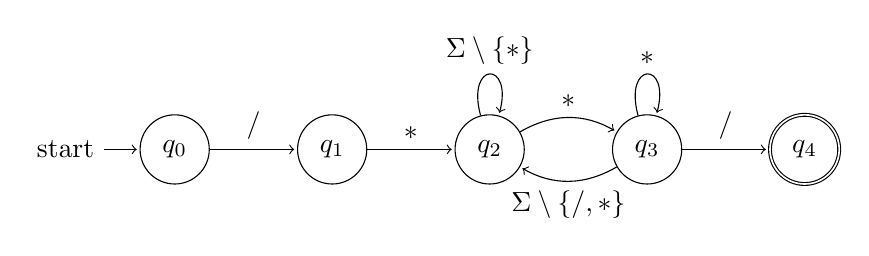
\begin{tikzpicture}[shorten >=1pt,node distance=2cm,on grid,auto]
		      \node[state,initial] (q_0) {$q_0$};
		      \node[state] (q_1) [right of=q_0] {$q_1$};
		      \node[state] (q_2) [right of=q_1] {$q_2$};
		      \node[state] (q_3) [right of=q_2] {$q_3$};
		      \node[state,accepting] (q_4) [right of=q_3] {$q_4$};

		      \path[->] (q_0) edge node {$/$} (q_1)
		                (q_1) edge node {$*$} (q_2)
		                (q_2) edge [bend left] node {$*$} (q_3)
		                edge [loop above] node {$\Sigma \setminus \{*\}$} ()
		                (q_3) edge [bend left] node {$\Sigma \setminus \{/,*\}$} (q_2)
		                edge [loop above] node {$*$} ()
		                edge node {$/$} (q_4);
		    \end{tikzpicture}
	    \end{center}
	    \caption{Example for a TikZ image; here using the \texttt{automata} library.}
	    \label{fig:tikz}
    \end{figure}
	Your first graphics in TikZ \emph{will} be time-eaters, but with some practice simple sketches are done in minutes.
	With a little bit of extra tuning, the same sources produce figures of unsurpassed quality.

  \item You can use document class \texttt{beamer} for creating presentation slides.
    It introduces some special syntax; best check the documentation and/or search the web.
\end{itemize}


\section{General research tools}

\begin{description}
	\item[\href{http://scholar.google.com}{Google Scholar} \& backwards search]
		~\\ % Cannot simply use \\ for newline as there would be an `empty' line ... therefore use ~\\
		Google Scholar can be used to find papers and books of all kinds and often has links to PDF versions that are freely available, e.\,g., on authors' websites.
		Moreover, Google Scholar can be used for finding other relevant articles in a field by backward-searching for papers that reference a given paper; see screenshot in Figure~\ref{fig:scholar}. % Use ~ for non-breaking space.
		Google Scholar has some basic support for exporting entries to BibTeX; the results often need some manual polishing, though.

		% Figures are placed by latex where they fit and should thus always be referenced by
		% the \label{}-\ref{} mechanism
		% \begin{figure}
		% 	\begin{center}
		% 		\fbox{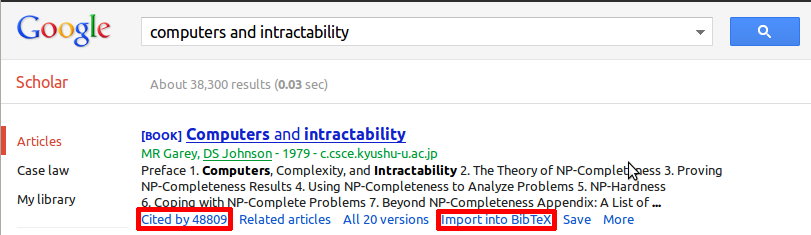
\includegraphics[width=.9\linewidth]{scholar}}%
		% 		% fbox for "framed box"
		% 	\end{center}
		% 	\caption{%
		% 		Some Google Scholar features we would like to highlight: back-references (find all papers that cite a given article) and BibTeX export (you may need to enable this in Google Scholar settings).
		% 	}
		% 	\label{fig:scholar} % NOTE: \label must appear after \caption
		% \end{figure}

	\item[\href{http://dblp.uni-trier.de/}{dblp}] is a searchable index of computer science bibliography with BibTex entries for all articles.

	\item[\href{http://www.mendeley.com}{Mendeley}] is a (free) web service for storing references (including PDFs).

		The collected references can be exported to BibTeX.

	\item[aspell] or some other spell checker.

		As a general rule, typos that can be found by running a spell checker are unacceptable.

	\item[Git] or some other version control system (like Subversion)

		Very useful for keeping old versions around and highly recommended.
		It works best on text files, but can also handle binary files.
		A comprehensive introduction is available as free ebook \cite{gitbook}.

		Git repositories can easily be cloned, e.\,g., onto an external drive for backup.
		That way, you get incremental backups of your work basically for free.

		As Git (and all other versioning systems) typically operate in a \emph{line-based} way,
		it is very advisable to break your text into short lines ($\approx$\,100 character).
		For documents that are edited collaboratively, it has been good practice to start a new line for each sentence (or even sub-clause)%
		\footnote{%
		  Recall that a newline is treated by \LaTeX{} like an ordinary space.
		  Only empty lines indicate a new paragraph.
		}.

\end{description}


\section{Bibliography}

%%%%%%%%%%%%%%%%%%%%%%%%%%%%%%%%%%%%%%%%%%%%%%%%%%%%%%%%%%%%%%%%%%%%%%%%%%%%%%%
\newpage
\nocite{*}
\bibliographystyle{eptcs}
\bibliography{references}

%%%%%%%%%%%%%%%%%%%%%%%%%%%%%%%%%%%%%%%%%%%%%%%%%%%%%%%%%%%%%%%%%%%%%%%%%%%%%%%
\end{document}
%%%%%%%%%%%%%%%%%%%%%%%%%%%%%%%%%%%%%%%%%%%%%%%%%%%%%%%%%%%%%%%%%%%%%%%%%%%%%%%
